\chapter[Results]{Results}
\label{kap:results}

In this chapter, we will take a look at the resulting data. We will also analyze the created probes and summarize the results of the thesis.  

%Spravila som nejaké grafy

\section{Partial results}

While searching for the final probes, we produced partial results, which include two sets of initial probes from which we picked probes to meet our requirements. 
We also created aligned data of the metal and nickel reference with both sets of probes and the aligned data for Odontarrhena tortuosa and Alyssum gmelinii probes. 
From those, we created the lists of probes to keep and to remove from the final result. 

\subsection{Initial probes}
We ran the Sondovač script with lowest possible minimum total locus length, which resulted into the highest possible number of probes. 
The script created $3628$ initial probes for Alyssum gmelinii and $9115$ initial probes for Odontarrhena tortuosa. 

There is signigicantly less probes for Alyssum gmelinii than for Odontarrhena tortuosa. While the quality of initial data for Alyssum gmelinii was better than for Odontarrhena, 
the sequencing methods differed and Alyssum has shorter reads (around 150bp). On the other hand, Odontarrhena has reads as long as 300bp, with much lower quality. Therefore, more 
probes were created from Odontarrhena reads, even if the quality is worse.  

While creating the probes, we ran the Sondovač script more times and found out the results are not the same. After additional investigation, we discovered that 
the results in fact, contain the same list of probes, but the order in which they are listed is different. The cause for this was probably FLASH or a difference in 
versions of Sondovač and software used. 


\subsection{Alignment}

We had five resulting files containing aligned sequences. 
The numbers of the matches were as follows: 
Alignment of Odontarrhena tortuosa probes and metal reference resulted in $286$ matches. Of these matches, $12$ probes had $90\%$ of the length aligned to the reference and $90\%$ similarity. 

Alignment of Odontarrhena tortuosa probes and nickel reference resulted in $112$ matches. None of these probes had $90\%$ of the length aligned to the reference and $90\%$ similarity. 

Alignment of Alyssum gmelinii probes and metal reference resulted in $248$ matches. None of these probes had $90\%$ of the length aligned to the reference and $90\%$ similarity. 

Alignment of Alyssum gmelinii probes and nickel reference resulted in $160$ matches. Of these matches, only one probea had $90\%$ of the length aligned to the reference and $90\%$ similarity. 

Alignment of Odontarrhena tortuosa probes and Alyssum gmelinii probes resulted in $586$ matches. None of these probes had $90\%$ similarity. 


Since we got so few results, for the specific requirements, we decided to gradually lower the required alignment length to see if there was a gap or some sort of a step, according to which we could 
say that from that alignment length, the sequences are truly aligned and not just a random occurence. 

\begin{figure}
\centerline{
	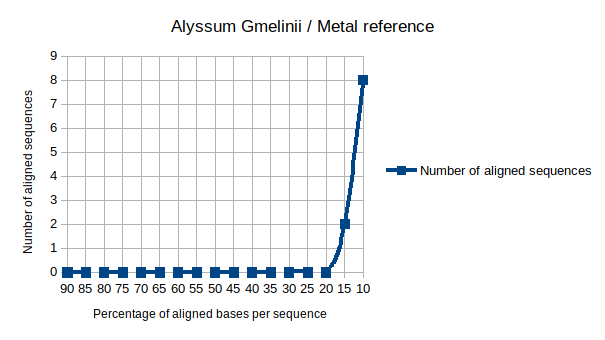
\includegraphics[width=0.7\textwidth]{images/gmelinii_metal.png}
}
\caption[Lowering of the required alignment length for succesful alignment]{Graph illustrating a number of alyssum gmelinii probes that had a similarity over $90\%$ while gradually lowering the required percentage of probe's aligned length when aligned to the metal reference.}
\label{obr:gmel_met}
\end{figure}

\begin{figure}
\centerline{
	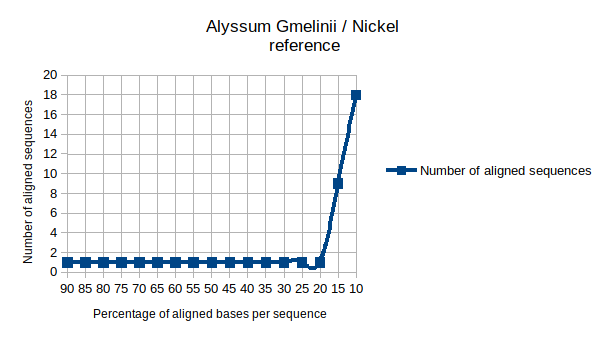
\includegraphics[width=0.7\textwidth]{images/gmelinii_nickel.png}
}
\caption[Lowering of the required alignment length for succesful alignment]{Graph illustrating a number of alyssum gmelinii probes that had a similarity over $90\%$ while gradually lowering the required percentage of probe's aligned length when aligned to the nickel reference.}
\label{obr:gmel_nick}
\end{figure}

\begin{figure}
\centerline{
	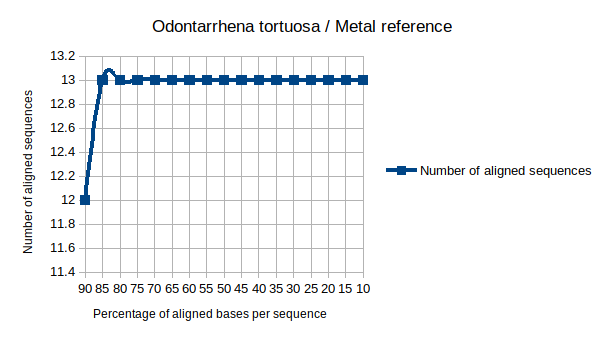
\includegraphics[width=0.7\textwidth]{images/odontarrhena_metal.png}
}
\caption[Lowering of the required alignment length for succesful alignment]{Graph illustrating a number of odontarrhena tortuosa probes that had a similarity over $90\%$ while gradually lowering the required percentage of probe's aligned length when aligned to the metal reference.}
\label{obr:odo_met}
\end{figure}

\begin{figure}
\centerline{
	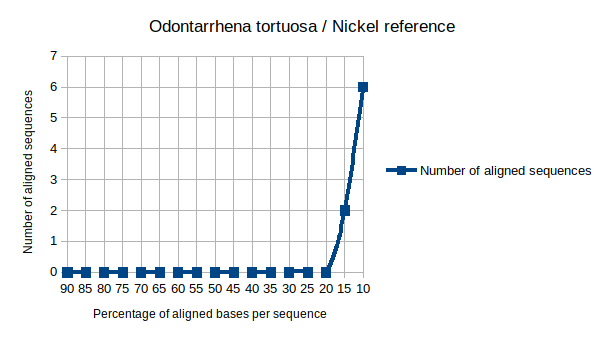
\includegraphics[width=0.7\textwidth]{images/odontarrhena_nickel.png}
}
\caption[Lowering of the required alignment length for succesful alignment]{Graph illustrating a number of odontarrhena tortuosa probes that had a similarity over $90\%$ while gradually lowering the required percentage of probe's aligned length when aligned to the nickel reference.}
\label{obr:odo_nick}
\end{figure}

Visual representation of these statistics didn't provide any more insight into the problem. 
Therefore, we tried to do the same thing, while lowering the required similarity. 

\begin{figure}
\centerline{
	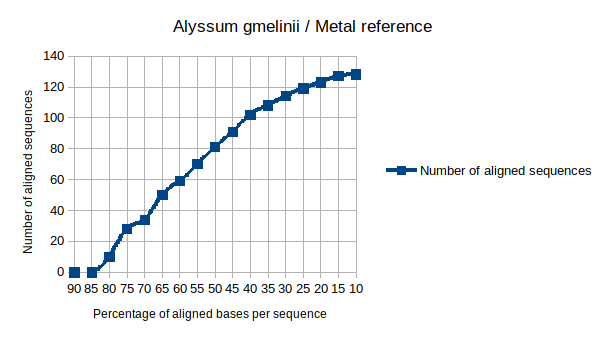
\includegraphics[width=0.7\textwidth]{images/gmelinii_metal_sim.png}
}
\caption[Lowering of the required alignment similarity for succesful alignment]{Graph illustrating a number of alyssum gmelinii probes that had an alignment length over $90\%$ while gradually lowering the required similarity of probe's alignment when aligned to the metal reference.}
\label{obr:gmel_met_sim}
\end{figure}

\begin{figure}
\centerline{
	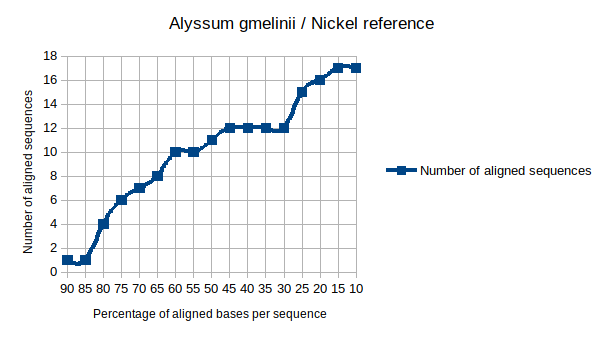
\includegraphics[width=0.7\textwidth]{images/gmelinii_nickel_sim.png}
}
\caption[Lowering of the required alignment similarity for succesful alignment]{Graph illustrating a number of alyssum gmelinii probes that had an alignment length over $90\%$ while gradually lowering the required similarity of probe's alignment when aligned to the nickel reference.}
\label{obr:gmel_nick_sim}
\end{figure}

\begin{figure}
\centerline{
	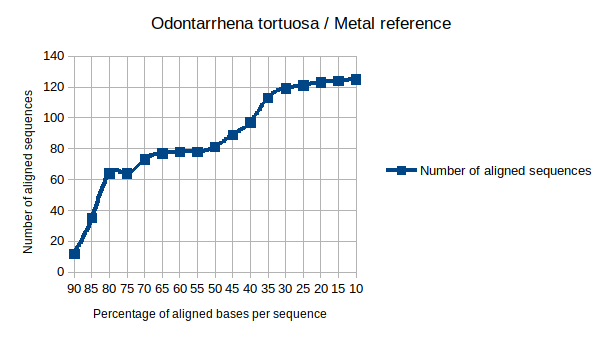
\includegraphics[width=0.7\textwidth]{images/odontarrhena_metal_sim.png}
}
\caption[Lowering of the required alignment similarity for succesful alignment]{Graph illustrating a number of odontarrhena tortuosa probes that had an alignment length over $90\%$ while gradually lowering the required similarity of probe's alignment when aligned to the metal reference.}
\label{obr:odo_met_sim}
\end{figure}

\begin{figure}
\centerline{
	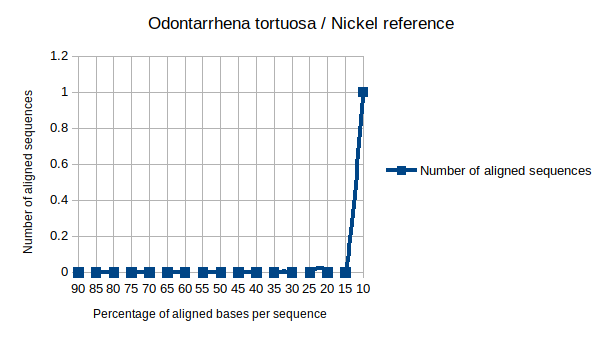
\includegraphics[width=0.7\textwidth]{images/odontarrhena_nickel_sim.png}
}
\caption[Lowering of the required alignment similarity for succesful alignment]{Graph illustrating a number of odontarrhena tortuosa probes that had an alignment length over $90\%$ while gradually lowering the required similarity of probe's alignment when aligned to the nickel reference.}
\label{obr:odo_nick_sim}
\end{figure}

However, the results varied so we we decided to include any matches LAST made, ordered by their similarity. 


\subsection{Probes to keep and remove}

Lists of probes to keep and to remove were produced. 
Unfortunately, in the script that created these lists, an error was made. The names of the files with these probes were exchanged, which caused the probes to keep to be removed and vice versa. 
This is a serious problem, because of which the probes might have to be made anew. 
%Napísať o zarovnaní prób, o hľadaní schodu, atď. 
%Že sa ich málo zarovnalo
%Napísať o vymenených súboroch

\section{Final probes}

Final probes were picked by a script and reached exactly $1,000,000$ base pairs as required. 

\subsection{Degenerated bases}

The final probes had to be edited and some of them replaced by another sequences, because many of them contained as much as $20\%$ of degenerated bases, which could pose a problem during hybridization of said probes. 
Therefore, we replaced any probes that contained more than $2.5\%$ of degenerated bases. This resulted in around $300$ sequences being replaced by other probes from the result that didn't contain degenerated bases. 

%Write about how many probes were created
%What happened to them. The problem with changed order and checking if they are the same set
%Write about masked nucleotides

